\section{Optimisations}

\begin{frame}
  \frametitle{The \lstinline{motionVectorSearch} algorithm}
  \begin{block}{Purpose}
    Reducing temporal redundancies between frames
    \onslide<+->
    \begin{itemize}
    \item<+-> I frame (encoded ``from scratch''): \alert{match frame}
    \item<+-> P frame (encoded using I frame, smaller): \alert{search
        frame}
    \end{itemize}
  \end{block}
  \onslide<+->
  \begin{exampleblock}{Steps}
    \begin{enumerate}
    \item<+-> select a \alert{match block} in the \alert{match
        frame} and its corresponding \alert{search window} in the
      \alert{search frame}
    \item<+-> loop over every \alert{search block} in the
      \alert{search window}
    \item<+-> find the \alert{search block} with the least \alert{SAD}
      from the \alert{match block}
    \item<+-> the \alert{motion vector} of the \alert{match block} is
      the position difference between it and the found \alert{search
        block}
    \end{enumerate}
  \end{exampleblock}
  \onslide<+->
  Three levels of loops to find the motion vector of every match
  block
\end{frame}

\begin{frame}
  \frametitle{Glossary of \lstinline{motionVectorSearch}}
  \begin{itemize}
  \item<1-> {\color{red} Red square}: match block
  \item<2-> {\color{blue} Blue square}: search window
  \item<3-> {\color{green} Green square}: search block
  \item<4-> {\color{brown} Brown arrow}: motion vector
  \end{itemize}
  \begin{figure}
    \centering
    \begin{subfigure}{.5\textwidth}
      \centering
      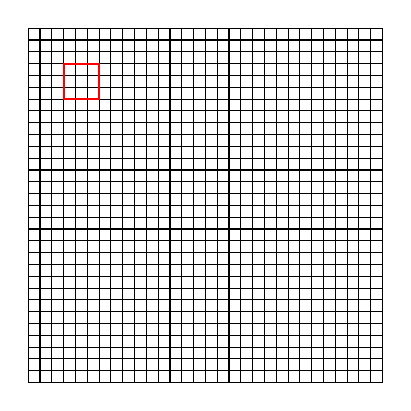
\begin{tikzpicture}[scale=0.15]
        \draw[step=1,black,thin] (0,0) grid (30,-30);
        \draw<1->[red,thick] (3,-3) rectangle (6,-6);
      \end{tikzpicture}
      \caption{Match frame}
    \end{subfigure}%
    \begin{subfigure}{.5\textwidth}
      \centering
      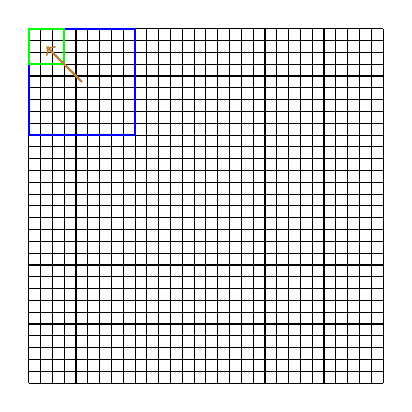
\begin{tikzpicture}[scale=0.15]
        \draw[step=1,black,thin] (0,0) grid (30,-30);
        \draw<2->[blue,thick] (0,0) rectangle (9,-9);
        \draw<3->[green,thick] (0,0) rectangle (3,-3);
        \draw<4->[brown,->,thick] (3+1.5,-3-1.5) -- (0+1.5,0-1.5);
      \end{tikzpicture}
      \caption{Search frame}
    \end{subfigure}
  \end{figure}
\end{frame}

\begin{frame}
  \frametitle{The inner loop of \lstinline{motionVectorSearch}}
  \begin{block}{Purpose}
    Measure the difference between \alert{match block} and
    \alert{search block}
  \end{block}
  \begin{figure}
    \centering
    \begin{subfigure}{.5\textwidth}
      \centering
      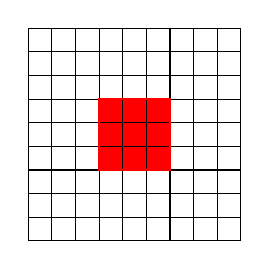
\begin{tikzpicture}[scale=0.3]
        \foreach \r in {0,...,2}{
          \foreach \c in {0,...,2}{
            \FPeval{\n}{clip(\r*3 + \c + 2)}
            \uncover<\n>{\fill[red] (3+\c, -3-\r) rectangle (3+\c+1, -3-\r-1);}
          }
        }
        \draw[step=1,black,thin] (0,0) grid (9,-9);
        \draw[step=1,red,thick] (3,-3) rectangle (6,-6);
      \end{tikzpicture}
      \caption{Match block}
    \end{subfigure}%
    \begin{subfigure}{.5\textwidth}
      \centering
      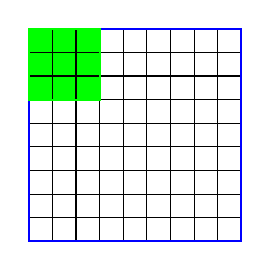
\begin{tikzpicture}[scale=0.3]
        \foreach \r in {0,...,2}{
          \foreach \c in {0,...,2}{
            \FPeval{\n}{clip(\r*3 + \c + 2)}
            \uncover<\n>{\fill[green] (\c, -\r) rectangle (\c+1, -\r-1);}
          }
        }
        \draw[step=1,black,thin] (0,0) grid (9,-9);
        \draw[blue,thick] (0,0) rectangle (9,-9);
        \draw[step=1,green,thick] (0,0) rectangle (3,-3);
      \end{tikzpicture}
      \caption{Search window}
    \end{subfigure}%
  \end{figure}
  \onslide<10->
  \begin{alertblock}{SAD}
    Sum of the absolute difference between the {\color{red} red} and
    {\color{green} green} filled squares
  \end{alertblock}
\end{frame}

\begin{frame}
  \frametitle{The middle loop \lstinline{motionVectorSearch}}
  \begin{block}{Purpose}
    Find the \alert{search block} with minimal \alert{SAD} in
    \alert{search window}
  \end{block}
  \begin{figure}
    \centering
    \begin{subfigure}{.5\textwidth}
      \centering
      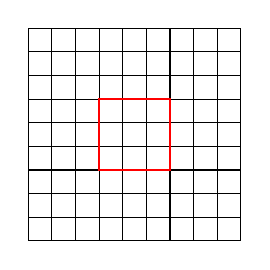
\begin{tikzpicture}[scale=0.3]
        \draw[step=1,black,thin] (0,0) grid (9,-9);
        \draw[red,thick] (3,-3) rectangle (6,-6);
      \end{tikzpicture}
      \caption{Match block}
    \end{subfigure}%
    \begin{subfigure}{.5\textwidth}
      \centering
      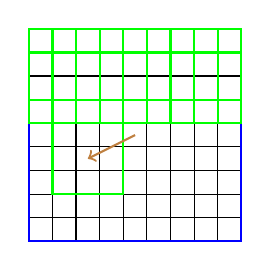
\begin{tikzpicture}[scale=0.3]
        \draw[step=1,black,thin] (0,0) grid (9,-9);
        \draw[blue,thick] (0,0) rectangle (9,-9);
        \foreach \r in {0,...,1}{
          \foreach \c in {0,...,6}{
            \FPeval{\n}{clip(\r*7 + \c + 1)}
            \uncover<\n>{\draw[green,thick] (\c,-\r) rectangle (3+\c,-3-\r);}
          }
        }
        \draw<15->[green,thick] (1,-4) rectangle (3+1,-3-4);
        \draw<16->[brown,thick,->] (4.5,-4.5) -- (2.5,-5.5);
      \end{tikzpicture}
      \caption{Search window}
    \end{subfigure}
  \end{figure}
  \onslide<16->
  \begin{alertblock}{Motion vector}
    The position difference between the \alert{match block} and its
    most similar \alert{search block} in \alert{search window}
  \end{alertblock}
\end{frame}

\begin{frame}
  \frametitle{The outer loop of \lstinline{motionVectorSearch}}
  \begin{block}{Purpose}
    Find the \alert{motion vector} for every \alert{match block}
  \end{block}
  \begin{figure}
    \centering
    \begin{subfigure}{.5\textwidth}
      \centering
      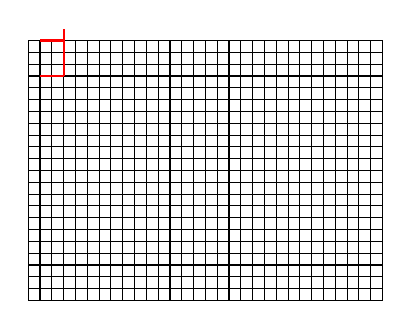
\begin{tikzpicture}[scale=0.15]
        \draw[step=1,black,thin] (0,0) grid (30,-22);
        \foreach \r in {1,...,2}{
          \foreach \c in {1,...,8}{
            \FPeval{\n}{clip((\r-1)*8 + \c)}
            \FPeval{\x}{clip(\c*3)}
            \FPeval{\y}{clip(-\r*3)}
            \uncover<\n>{\draw[step=3,red,thick] (\x,\y) grid (\x+3,\y-3);}
          }
        }
      \end{tikzpicture}
      \caption{Match frame}
    \end{subfigure}%
    \begin{subfigure}{.5\textwidth}
      \centering
      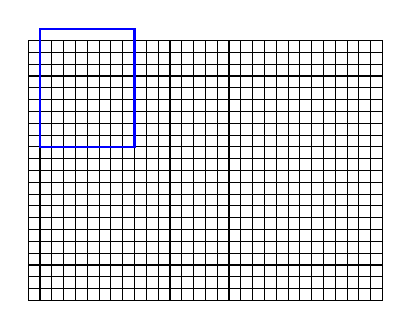
\begin{tikzpicture}[scale=0.15]
        \draw[step=1,black,thin] (0,0) grid (30,-22);
        \foreach \r in {0,...,1}{
          \foreach \c in {0,...,7}{
            \FPeval{\n}{clip(\r*8 + \c + 1)}
            \FPeval{\x}{clip(\c*3)}
            \FPeval{\y}{clip(-\r*3)}
            \uncover<\n>{\draw[blue,thick] (\x,\y) rectangle (\x+9,\y-9);}
          }
        }
      \end{tikzpicture}
      \caption{Search frame}
    \end{subfigure}
  \end{figure}
  \onslide<16->
  \begin{alertblock}{Output}
    An array of \alert{motion vectors}
  \end{alertblock}
\end{frame}

\begin{frame}
  \frametitle{Analysing \lstinline{motionVectorSearch}}
  \begin{block}{Properties}
    \begin{itemize}
    \item<+-> Task dependency only within group (finding min SAD)
    \item<+-> Computational intensity \(> \frac{3_{op} \times (16 \times 16)_{InnerLoop} \times
        (33 \times 33)_{MiddleLoop} \times (254 \times 254)_{OuterLoop}}{(4096 \times
        4096)_{FrameSize} \times 4_{byte}} = 804\) OP/B
    \item<+-> \((33 \times 33)_{MiddleLoop} \times (254 \times 254)_{OuterLoop} =
      65605\) parallelisable tasks
    \end{itemize}
  \end{block}
  \onslide<+->
  \begin{figure}[h]
    \centering
    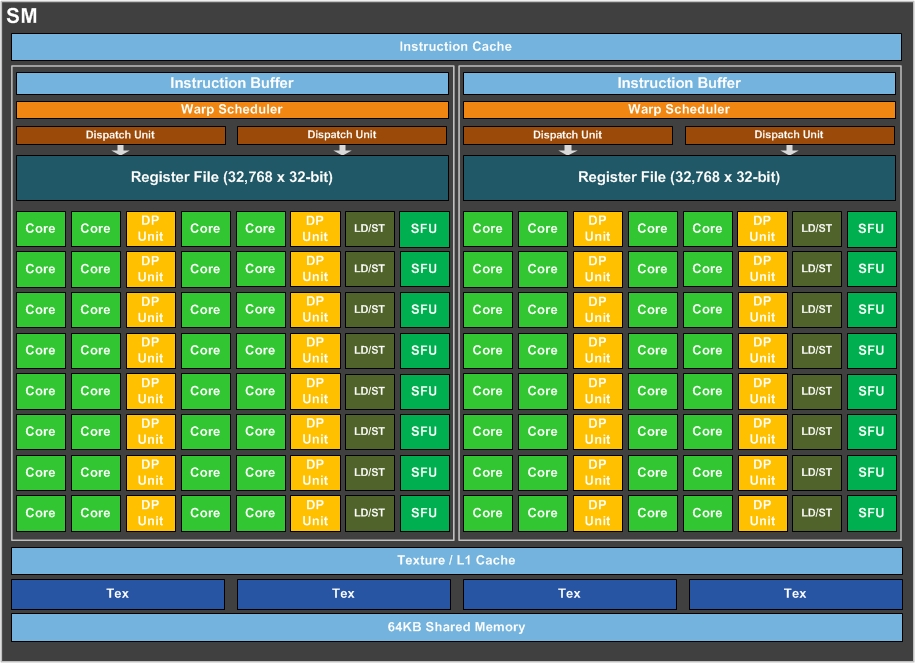
\includegraphics[height=2cm]{sm.png}
    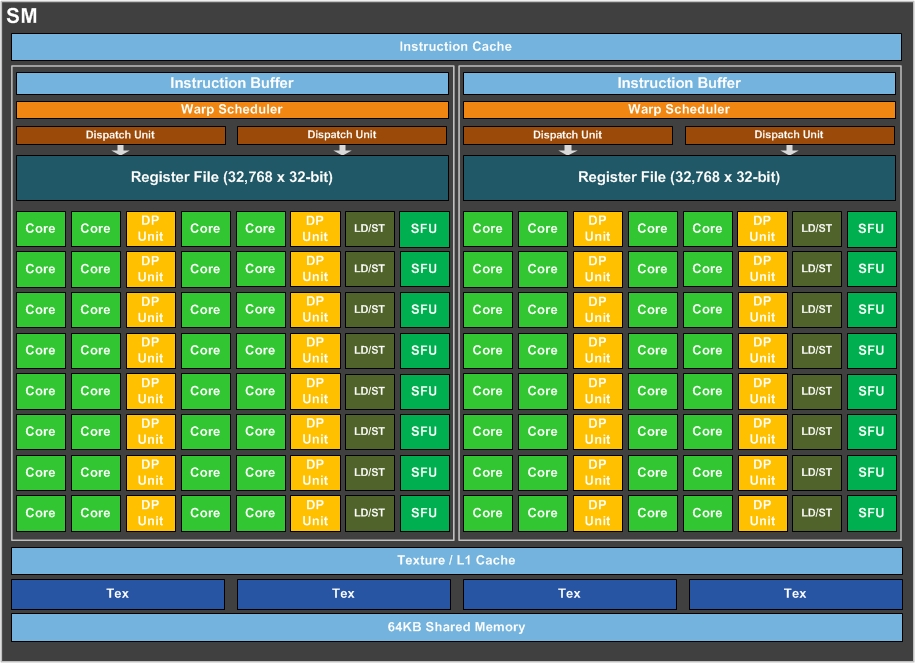
\includegraphics[height=2cm]{sm.png}
    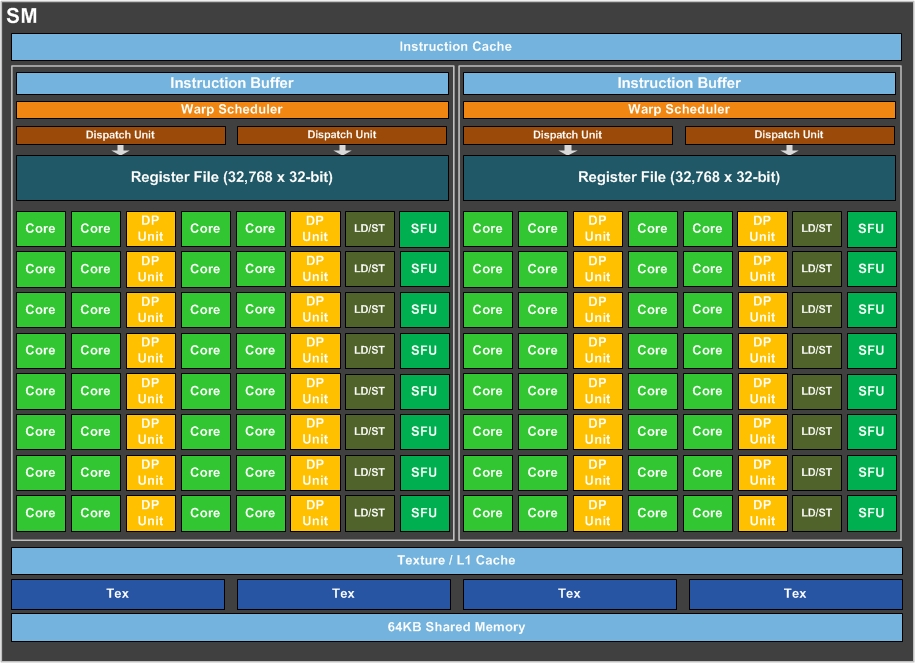
\includegraphics[height=2cm]{sm.png}
  \end{figure}
  \onslide<+->
  \begin{alertblock}{Decision}
    Perfect computation for GPU
  \end{alertblock}
\end{frame}

\begin{frame}
  \frametitle{OpenCL work groups for \lstinline{motionVectorSearch}
    kernel}
  \begin{block}{Why groups}
    \begin{itemize}
    \item<+-> Each work group finds the \alert{motion vector} for a
      \alert{match block}
    \item<+-> Finding min \alert{SAD} requires synchronisation
    \end{itemize}
  \end{block}
  \begin{figure}
    \centering
    \begin{subfigure}{.5\textwidth}
      \centering
      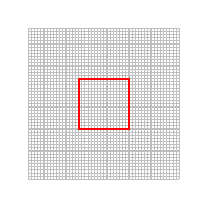
\begin{tikzpicture}[scale=0.04]
        \draw[step=1,lightgray,thin] (0,0) grid (48,-48);
        \draw[red,thick] (16,-16) rectangle (32,-32);
      \end{tikzpicture}
      \caption{Match block}
    \end{subfigure}%
    \begin{subfigure}{.5\textwidth}
      \centering
      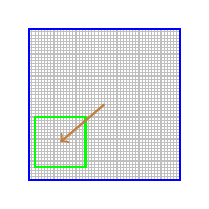
\begin{tikzpicture}[scale=0.04]
        \draw[step=1,lightgray,thin] (0,0) grid (48,-48);
        \draw[blue,thick] (0,0) rectangle (48,-48);
        \draw[green,thick] (2,-28) rectangle (16+2,-16-28);
        \draw[brown,thick,->] (24,-24) -- (10,-36);
      \end{tikzpicture}
      \caption{Search window}
    \end{subfigure}
  \end{figure}
  \onslide<+->
  \begin{alertblock}{Dimensions}
    \begin{itemize}
    \item<+-> Global dimensions: \(4096 \times 4096\)
    \item<+-> Local dimensions: \(16 \times 16\)
    \end{itemize}
  \end{alertblock}
\end{frame}

\begin{frame}
  \frametitle{Signature and edge blocks of
    \lstinline{motionVectorSearch} kernel}
  \begin{block}{Parameters}
    \begin{itemize}
    \item \lstinline{sy, scb, scr} are channels of the search frame
    \item \lstinline{my, mcb, mcr} are channels of the match frame
    \item \lstinline{out} is the output array of motion vectors
    \end{itemize}
  \end{block}
  \begin{exampleblock}{}
    \lstinputlisting[basicstyle=\tiny,linerange=15-25]{src/kernel.cl}
  \end{exampleblock}
  \begin{alertblock}{}
    The work groups on the edges do nothing
  \end{alertblock}
\end{frame}

\begin{frame}
  \frametitle{Utilising local memory for
    \lstinline{motionVectorSearch} kernel}
  \begin{block}{Why local memory}
    \begin{itemize}
    \item<+-> Reuse every element multiple times
    \item<+-> Some group local variables for reduction
    \end{itemize}
  \end{block}
  \onslide <+->
  \begin{exampleblock}{}
    \lstinputlisting[basicstyle=\tiny,linerange=27-30]{src/kernel.cl}
  \end{exampleblock}
  \onslide <+->
  Fits pretty well (max \(49152_{Byte}\))
  \begin{align*}
    search &= (48 \times 48)_{SearchFrameSize} \times 3_{Channel} \times
             4_{Byte} = 27648_{Byte}\\
    match &= (16 \times 16)_{MatchFrameSize} \times 3_{Channel} \times
            4_{Byte} = 3072_{Byte} \\
    sad &= (16 \times 16)_{BlockSize} \times 4_{Byte} = 1024_{Byte} \\
    motion &= (16 \times 16)_{BlockSize} \times 8_{Byte} = 2048_{Byte} \\
    Total &= 33792_{Byte}
  \end{align*}
\end{frame}

\begin{frame}
  \frametitle{Load to local memory for \lstinline{motionVectorSearch}
    kernel}
  \begin{exampleblock}{}
    \lstinputlisting[basicstyle=\tiny,linerange=32-53]{src/kernel.cl}
    {\color{red} \lstinputlisting[basicstyle=\tiny,linerange=55-55]{src/kernel.cl}}
  \end{exampleblock}
\end{frame}

\begin{frame}
  \frametitle{Compute SAD for \lstinline{motionVectorSearch} kernel}
  \framesubtitle{Part 1}
  \begin{exampleblock}{}
    \lstinputlisting[basicstyle=\tiny,linerange=57-69]{src/kernel.cl}
    \qquad \qquad {\color{red} Part 2}
    \lstinputlisting[basicstyle=\tiny,linerange=94-98]{src/kernel.cl}
  \end{exampleblock}
\end{frame}

\begin{frame}
  \frametitle{Compute SAD for \lstinline{motionVectorSearch} kernel}
  \framesubtitle{Part 2}
  \begin{exampleblock}{}
    \lstinputlisting[basicstyle=\tiny,linerange=70-93]{src/kernel.cl}
  \end{exampleblock}
\end{frame}

\begin{frame}
  \frametitle{Find the min SAD motion vector for
    \lstinline{motionVectorSearch} kernel}
  \begin{exampleblock}{}
    \lstinputlisting[basicstyle=\tiny,linerange=99-119]{src/kernel.cl}
  \end{exampleblock}
\end{frame}

\begin{frame}
  \frametitle{Results of optimising \lstinline{motionVectorSearch}}
  \begin{alertblock}{Average time improvement}
    \begin{itemize}
    \item<+-> \(500000_{ms} \to 500_{ms}\)
    \item<+-> 1000x speedup
    \end{itemize}
  \end{alertblock}
\end{frame}


%%% Local Variables:
%%% mode: latex
%%% TeX-master: "presentation"
%%% End:
